%!TEX root = ./../main.tex
\chapter{Introduction}
% Parte introduttiva dall'A di federica; obbiettivi:
% capire quanto accurata la descrizione Ele CG per ottenere risultati giusti rispetto all'atomistico; complicazione relative all'interazione ele, si sono già affrontati con martini STD cg.
%
% Richiamo a due risultati exp in contraddizione: fig 2 federica con il lavoro di reflettometria a neutroni, Macchirini. Contraddizione -> Simulazioni MD per capire cosa succede meglio
%
% D federica
%
% Stato dell'arte di conti di energia libera di soluti che penetrano in membrana

\begingroup
%necessary for tocless section
\toclesssection
\introductionStyle

\section{motivations}
Metal \acp{NP} play more and more important roles in pharmaceutical and medical technology as diagnostic or therapeutic devices. Metal \acp{NP} can nowadays be engineered in a multitude of shapes, sizes and compositions, and they can be decorated with an almost infinite variety of functionalities. Despite such technological advances, there is still poor understanding of the molecular processes that drive the interactions of metal \acp{NP} with cells. Cell membranes are the first barrier encountered by \acp{NP} entering living organisms. The understanding and control of the interaction of \acp{NP} with biological membranes is therefore of paramount importance to understand the molecular basis of the \acp{NP} biological effects.

The overall goal of this thesis is to elucidate which molecular mechanisms take place during the \ac{NP}--membrane interaction and, from a purely methodological standpoint, indicate which models of atomic and molecular interactions are appropriate to achieve this goal via classical \ac{MD} simulations.

We will now draw the background scenario of the thesis, going more into detail about our motivations and the state of the art of the computational studies in this field.

% This thesis is focused on the study of the interaction between ligand--protected anionic \acp{AuNP} and model biological membranes via computational means. Our first aim is to understand how the description of the electrostatic interaction have to be accurate, at \ac{CG} level, in order to obtain quantitative results approaching the atomistic model, in less computational time. A second objective is the estimation of the free energy barriers associated to the transitions involved in the \ac{NP}--membrane interaction using a \ac{CG} \ac{FF} (see chapter~\ref{chap:EmpiricalFF}). Moreover it is important to characterize, at molecular--level, the \ac{NP}--membrane interaction and the structural deformation of the bilayer in presence of the \ac{NP}.
%: how does the passive \ac{NP}-membrane interaction happen? What are the physical driving forces leading to the formation of a stable \ac{NP}-membrane complex (electrostatic interactions, hydrophobic interactions...)? How does the composition of the \ac{NP} ligand shell affects such an interaction?


\section{relevant experimental results and NP--membrane interaction issues}
Membrane permeation can happen via direct translocation, which is a passive mechanism, or via endocytosis, which on the contrary is an active, receptor--mediated process. Direct translocation is more likely for small ($< 10$~nm) \acp{NP}, while the endocytotic pathway is typical of the larger ones.

Depending on the target application, the \ac{NP} may be required to easily, passively go through the cell membrane, or to bind to specific receptors and enter the cell via a protein--mediated pathway, or even to stably bind to the membrane. The membrane--\ac{NP} interaction results from the complex interplay of electrostatics, hydrophobic interactions, ligand composition, surface ligand organization and, on the membrane side, lipid composition and phase.

In particular it is known form literature that the charge of the surface ligands plays an important role in the toxicity of the functionalized \ac{NP} interacting with lipid membrane. Goodman \etal in \cite{Goodman2004}, via experiment on living cels and bacterial cultures and fluorescence microscopy using multilamellar neutral lipid vesicles, have found that the toxicity mechanism is related to the formation of pores in the membrane that can lead to membrane destruction. Moreover, they found that cationic \acp{AuNP} are more destructive than the anionic one, as we can see from figure~(\ref{fig:goodman}).
\begin{figure}[!ht]
	\centering
	\subfloat[]{%
		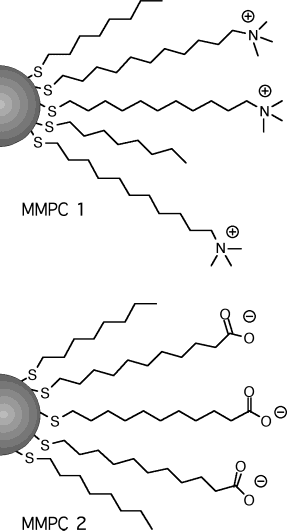
\includegraphics[width=0.2\textwidth]{./img/GoodmanNPs.png}%
	}\qquad\qquad%
	\subfloat[]{%
		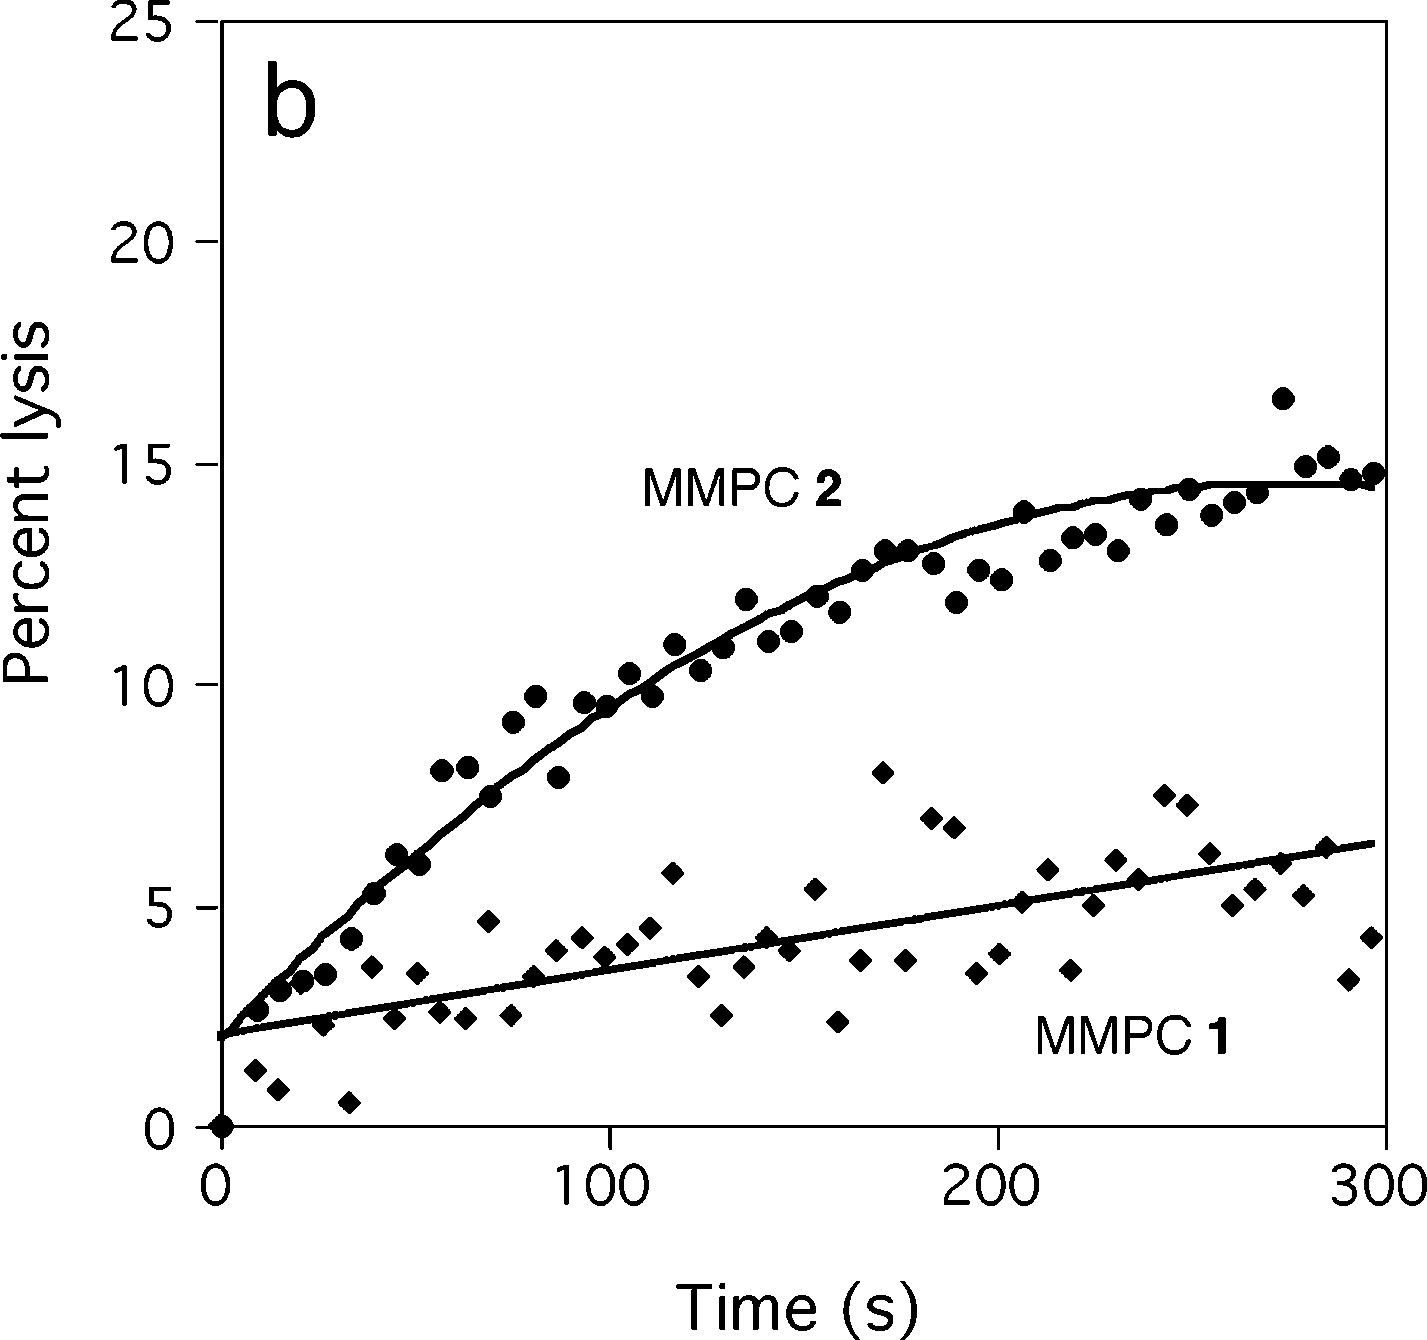
\includegraphics[width=0.4\textwidth]{./img/lysis.png}%
	}%
	\caption{Left: \acp{AuNP} functionalized by a monolayer of neutral and positively charged (MMPC $1$) or negatively charged (MMPC $2$) ligands. Right: Comparison of MMPC $1$ and $2$ in disrupting vesicles made of neutral lipids. In this kind of essays, the disruptive power of the \acp{NP} is quantified by the amount of fluorescent dye that is released from the vesicles. Taken from \cite{Goodman2004}.}%
	\label{fig:goodman}
\end{figure}

More recently, Van Lehn \etal \cite{VanLehn2013} from experimental results via confocal microscopy images, shown in figure~(\ref{fig:fluorescent}), have demonstrated that anionic \acp{AuNP} can stably bind to the lipid membrane in a non--destructive manner and moreover that they can passively diffuse inside a multilamellar vesicle made of a zwitterionic lipid. The \ac{AuNP} was labelled with the red fluorescent BODIPY dye and solved in a water solution with the multilamellar vesicle and a green fluorescent calcein dye that does not passively diffuse through lipid bilayers.
\begin{figure}[!ht]
	\centering
	\subfloat[calcein fluorescence]{%
		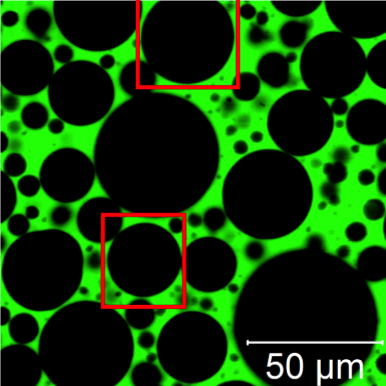
\includegraphics[width=0.28\textwidth]{./img/Calcein.png}%
	}\qquad\qquad\qquad%
	\subfloat[BODIPY fluorescence]{%
		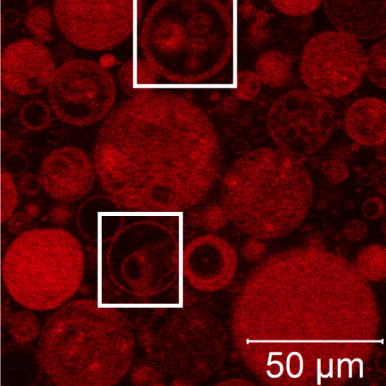
\includegraphics[width=0.28\textwidth]{./img/BODIPY.png}%
	}%
	\caption{Confocal microscopy images of BODIPY--labeled anionic \acp{AuNP} in a solution with multilamellar single--component zwitterionic lipid vesicles and the membrane impermeable dye calcein. Green fluorescence from calcein, left image, was only observed from the vesicle exterior. This means that no vesicles has been destroyed since the calcein can penetrate the vesicle interior only if pores are formed in the lipid membrane. Indicating that anionic \acs{AuNP} do not induce pore formation. BODIPY red fluorescence, right image, was localized to both interior and exterior membranes of the multilamellar vesicles, with a noticeably stronger fluorescence at the interior respect to the background. This suggest a preferential bilayer--\acs{AuNP} interaction and that the \acp{AuNP} can passively diffuse through the lipid membrane in a non--destructive manner. Taken from \cite{VanLehn2013}.}%
	\label{fig:fluorescent}
\end{figure}

In another recent work, Tatur \etal \cite{Maccarini2013}, made a neutron reflectometry experiment on a floating zwitterionic lipid bilayer in presence of \acp{AuNP} functionalized with both anionic and cationic ligands. Studying the structural deformation of the bilayer they found that the cationic \acs{NP} are overall more toxic then the anionic one. They found that the latter can passively penetrate into the hydrophobic region of the membrane in a non destructive manner for wide range of temperatures under the liquid--gel transition. Above the liquid--gel transition, instead, they observe that more and more cationic \acp{NP} can permanently penetrate inside the membrane leading to a gradual destabilization of its structure, depending on the quantity of inserted \acp{AuNP}. On the contrary, the anionic \acp{AuNP} do not have the tendency to penetrate inside the lipid membrane. Rather, they interact with its surface strongly dehydrating the floating bilayer. As a consequence the authors suggest a possible decrease in the bilayer thickness and an increase of its susceptibility to disintegrate and to form lipid vesicles. Clearly these results are in contrast with the confocal microscopy observation reported in Van Lehn \etal \cite{VanLehn2013}. Hence the importance to perform \ac{MD} simulations to investigate the molecular processes involved in the \ac{NP}--membrane interaction.

Other physico--chemical characteristics of the \ac{NP} ligand shell affect the \ac{NP}--membrane interaction. On top of all, the hydrophobic character of the ligand shell is believed to play a major role. Moreover, what is most intriguing and unexplained is the effect of the ligand composition and surface arrangement on the \ac{NP}--membrane interaction. To date, neither the poration process, nor the binding process, nor the effects of ligands with different degrees of hydrophobicity have been described at molecular level, hindering the design of \acp{NP} with target--specific ligand composition.


\section{state of the art of the computational studies of aunp--lipid membrane interactions}
Van Lehn \etal have published a computational work \cite{VanLehn2013} concerning the way anionic \acp{NP} penetrate cells membrane. They studied the influence of the size and surface composition of functionalized \acp{AuNP} on the internalization pathway into the cells in addition to the steps through which the process evolves. They used both a thermodynamic--based model and experiments, see figure~(\ref{fig:fluorescent}), to test the hypothesis that the first step in cells penetration is the fusion of the \acp{AuNP} with lipid bilayers, the process being driven by the hydrophobic effect. The hypothesized mechanism relies on the capability of the ligands on the \ac{NP} surface to ``snorkel'' the charged end groups to the aqueous environment thus exposing a greater hydrophobic area to the bilayer core. Van Lehn \etal conclude that the process is size--dependent rather than morphology--dependent and that there exists a critical diameter, dependent on the coating composition, above which fusion with the lipid bilayer becomes unfavorable.

Heikkilä \etal in \cite{Heikkila2014} demonstrated, by \ac{MD} simulations, that anionic \acp{AuNP} can adsorb at the surface of neutral lipid membranes. The limited time scale of the simulations performed in their work, which is based on an atomistic \ac{FF} (see chapter~\ref{chap:EmpiricalFF}), did not allow to observe and describe any penetration of the \ac{NP} into the hydrophobic membrane core. To speed--up the process, Van Lehn \etal in \cite{VanLehn2014} have considered the interaction between an anionic \ac{AuNP} and a highly curved lipid bilayer, observing the fusion between the \ac{NP} and the membrane.

Gkeka \etal modelled rigid \cite{Gkeka2013} and \ac{CG} \cite{Gkeka2014} (see chapter~\ref{chap:EmpiricalFF}) \acp{NP}, with different arrangements of the charged surface ligands, in the attempt of deriving free energies of transfer from the water phase to the membrane interior for \acp{NP} with different degrees of hydrophobicity.

More recently, in order to speed--up the unbiased \ac{MD} simulation and the \ac{NP}--membrane interaction, Federica Simonelli \etal \cite{simonelliThesis} and \cite{ourPaper}, have developed a \ac{CG} model of the anionic, passivated \ac{AuNP} (see chapter~\ref{chap:membraneNP}). The enhancement of the computational performance, thanks to the \ac{CG} model, allowed to derive, via unbiased \ac{MD} simulations, the molecular mechanism associated to the interaction between the \ac{NP} and a planar model biological membrane. Furthermore they found that the \ac{NP}--membrane interaction depends on the surface arrangements of the \ac{NP} ligands.
%Second, to perform a preliminary free energy profile of transfer of one charged ligands form the entrance leaflet to the opposite one.

% \section{state of the art of the free energy calculations on lipid membrane solutes translocation}
% Free energy calculations refers to the possibility, via advanced sampling methods, to obtain thermodynamic results of processes or transitions between two metastable states that have low probability to occur in an \textit{unbiased} \ac{MD} simulation at a certain temperature. As better explained in chapter~\ref{chap:methods} advanced sampling methods force --- via the introduction of a bias force --- the sampling of the non--accessible phase space. Advanced sampling methods allow to accelerate rare events, and so simulate them within accessible time scales, and to provide a quantitative description of the \ac{FES} in the region of interest of the phase space. A simple example involving lipid membranes is the ion translocation through the bilayer from the water phase: the advanced sampling methods allow for the extremely unlikely process to occur and, as accurately as possible, for the estimation of the free energy profile. To do this a \ac{CV} or an order parameter, a variable or a set of variables that describes the process of interest, are necessary in order to integrate out the other, supposed, unnecessary \ac{DOF}. In the above example and in those cases in which the process of interest is a solute translocation through a lipid bilayer, the most intuitive and commonly--used \ac{CV} is the distance between the \ac{COM} of the solute and the \ac{COM} of the lipid membrane along the bilayer normal. Unfortunately, in most cases this \ac{CV} is the origin of some sampling error and a non correct estimation of the \ac{FES}, as outline in a review by by Neale and Pomès \cite{Neale2016}.

% In the following we summarize the main concepts useful for this thesis work, for a more comprehensive discussion the reader is addressed to the review by Neale and Pomès \cite{Neale2016}.

%The sampling errors, which often are systematic, arise when large free energy barriers in orthogonal degrees of freedom, also called hidden free energy barriers, trap the sampling in a undesired metastable states. In the lipid membrane solutes translocation, the common hidden energy barriers are due to deformations of one or both leaflets. There are two main kind of deformations: an invagination of the bilayer around the solute, as shown in figure~(\ref{fig:hfes}) or a deformation of one or both leaflets due to the interaction between the charged lipid heads and the charged solute groups (and its hydration shell), as shown in figure~(\ref{fig:invaginatino}). In the last effect, the solute, bringing water and lipid head groups of one or both leaflet can create a membrane defect that can lead to a water pore formation. %The invagination or the deformation of one or both leaflets of the bilayer upon solute penetration implies that the free energy cost of desolvating ionic solutes exceeds the cost of bilayer deformation and hence that the magnitude of the free energy barrier of the entrance process depends to a large extent on the bilayer's thickness and bending modulus.
% \begin{figure}[ht!]
% 	\centering
% 	\subfloat[]{%
% 		\begin{minipage}[c][1\width]{0.4\textwidth}%
% 			\centering%
% 			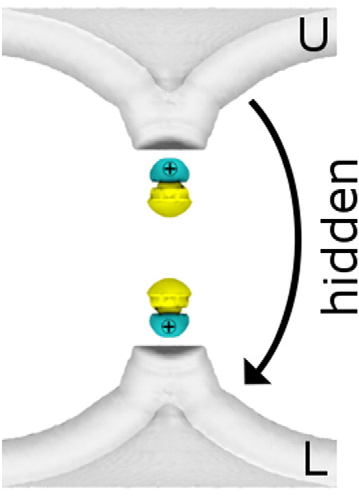
\includegraphics[width=0.6\textwidth]{./img/HFES.png}%
% 			\label{fig:hfes}%
% 		\end{minipage}%
% 	}\qquad%
% 	\subfloat[]{%
% 		\begin{minipage}[c][1\width]{0.4\textwidth}%
% 			\centering%
% 			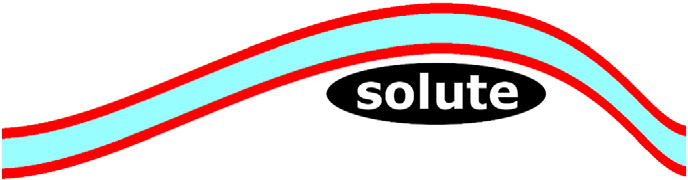
\includegraphics[width=\textwidth]{./img/invagination.png}%
% 			\label{fig:invaginatino}%
% 		\end{minipage}%
% 	}%
% 	\caption{Bilayer distortion and hidden free energy barriers underlying systematic sampling errors in free energy calculations. (a) Example of both leaflets trailing towards the bilayer core due the translocating solute. In gray the phosphorus atoms behind the solute and yellow hydrophobic and cyan hydrophilic moieties of the solute. The curved arrow indicate the hidden energy barriers. (b) Example of a possible invagination of the lipid membrane around the solute; the \acs{COM} of the solute and the lipid bilayer coincide but the solute is still in the water phase. Taken from \cite{Neale2016}.}%
% \end{figure}

%The invagination effect, that can be caused also by a sufficiently large bilayer, can cause false associations between the \ac{CV} and the state of the system. As shown in figure~(\ref{fig:invaginatino}) defining the \ac{CV} as the distance between the \ac{COM} of the solute and the bilayer, $|z|$, a solute at $|z| = 0$ may not for a direct contact with the core of the bilayer, there by sampling an irrelevant region of phase space and yielding a free energy profile with no real predictive value.

%The main force acting on a charged solute embedded near the bilayer center is largely determined by the presence of a defect that brings water and lipid head groups of one or both leaflets into the bilayer's hydrophobic core. Therefore, the extent to which the free energy profile of translocation is affected by sampling errors depends on the free energy of defect formation for a given \ac{FF}. Unexpectedly, the likelihood of forming such defects, which is intricately tied to the bilayer's bending modulus, can depend on the way the non--bonded interactions are modelled. In the common case of a Lennard--Jones potential, it depend, therefor, in the used truncation methods.

%By far the most commonly used \ac{CV} in free energy simulations of solute--bilayer interactions is the distance between the \ac{COM} of the solute and that of the bilayer along the bilayer normal. The existence of persistent systematic sampling errors, as seen above, demonstrates that this commonly--used order parameter is inadequate for many free energy calculations. However, the selection of the optimal \acp{CV} set is a challenging problem that deserves a more appropriate studies for understand if the set of \acp{CV} are useful to describe the process and how it impact the computational performance of the simulation: a incredible perfect set of \acp{CV} that slow down the simulation can not be useful. For this and for a comparison between the results obtained in \cite{ourPaper} to be made, for this thesis work, we have chosen to not change the selected \ac{CV}, based on the distance between the \ac{COM} of the solute and the membrane along the bilayer normal.

\section{objectives}
In the previous paragraphs we have highlighted two main challenges related to the study of charged metal \ac{NP}--membrane interactions. The first consists in the difficulty to achieve experimentally a molecular--level description of the \ac{NP}--membrane interaction. This issue could be in principle be addressed computationally, but the second difficulty soon kicks in --- at computational level the \ac{NP}--membrane interaction is a ``slow'' process, and it is not trivial to achieve the optimum compromise between the model reliability and computational efficiency.

Here we list the three main objectives of this thesis:
\begin{enumerate}[label=\itshape\roman*.]
	\item Do anionic \acp{NP} bind to neutral, zwitterionic lipid membranes? If they do, can we use \ac{MD} simulations to reveal the molecular mechanisms that lead to \ac{NP}--membrane binding, and can we make quantitative predictions about the strength of the \ac{NP}--membrane interactions?%
	\item The \ac{NP}--membrane interaction is driven by two main physical causes: \textit{a.} the hydrophobic effect, that favors the hydrophobic contacts between the \ac{NP} and the membrane, and \textit{b.} electrostatic interactions, that favor the contact between the anionic \ac{NP} ligands and the neutral, but polar, heads of the lipid molecules. The role played by electrostatics is important, but electrostatic interactions are not always properly taken into account by the classical interaction models used in biomolecular simulations. All--atom models typically include the description of long--range electrostatics and the molecular orientational polarizability, but are extremely expensive from a computational point of view. \ac{CG} models, on the contrary, are computationally efficient but often inaccurate at the description of the interaction between charged or polar molecules. Our aim is to compare these different approaches and suggest what model allows for the best compromise between computational efficiency and reliability.%
	\item In presence of mixed--ligand shells, can the surface arrangement of ligands influence the \ac{NP} interaction with the membrane? Our objective is to consider \acp{NP} passivated with a mixed shell of hydrophobic and anionic ligands. We will look at \acp{NP} in which the two kinds of ligands have an ordered (striped--like) arrangement of the two ligands, and \acp{NP} with a random ligand arrangement. In both cases we will characterize the \ac{NP}--membrane interaction mechanism and compare the \ac{NP}--membrane binding energies of the two samples.%
\end{enumerate}

\section{contents overview}
In this thesis we characterize the interactions between an anionic, ligand--protected \ac{AuNP} and a model lipid membrane by means of \ac{MD} simulations and an enhanced sampling method, called metadynamics. Both \ac{MD} and metadynamics's main features are described in chapter~\ref{chap:methods}.

%\ac{MD} is a numerical scheme used to integrate the equations of motion for systems made of particles which can be identified with atoms, molecules or even larger groups of atoms. Metadynamics is a method and a sort of \ac{MD} plug--in that allow free energy calculations, for the estimation of the free energy profile and to enhance the probability of a rare events to occur. They main features are described in chapter~\ref{chap:methods}.

The choice of the appropriate model of inter-particle interactions to feed the \ac{MD} method depends on the typical time and length scales of the system of interest. The stages of the \ac{NP}--membrane interaction --- from the water phase to the \ac{NP} embedded into the lipid membrane  --- take place on time scales of at least tens of microseconds. In terms of length scales, the size of the membrane patch to be considered in our simulations needs to be as large as $10$~nm at least, in order to be able to accommodate a \ac{NP} which metal core has a diameter of about $2$~nm. These time and length scales are not compatible with the use of an atomistic \ac{FF}, that is, a model interaction potential describing the interactions between all the atoms in the system. We thus adopted a \ac{CG} approach, based on the idea that groups of atoms (e.g. the charged terminal group of an anionic ligand, or the polar head of a lipid) can be represented by single particles. A general introduction and features about \ac{FF}, the advantages (and disadvantages) of a \ac{CG} \ac{FF} over an atomistic one and a detail description of the \ac{CG} \ac{FF} that I will use are described in the first part of chapter~\ref{chap:EmpiricalFF}. Since we are interested in improving the treatment of the electrostatic interaction, in the second part of chapter~\ref{chap:EmpiricalFF} we present two methods to efficiently and accurately treat the electrostatic interaction: the \ac{ESM} and the \ac{PME} method.

In chapter~\ref{chap:software} we present a general overview of the software tools used in this work. Moreover, some computational tricks and tips used to improve the computational perforce of my \ac{MD} runs are presented. The main one is the use of an hardware accelerated framework for off--loading the non--bonded calculation and achieve a speed--up of about $2-4$ times respect to non accelerated simulation.

In chapter~\ref{chap:membraneNP} we present the main properties of the \ac{CG} model of the biological lipid membrane and the \ac{CG} model of the anionic, ligand--passivated \ac{AuNP} developed by Federica Simonelli \etal \cite{simonelliThesis} and \cite{ourPaper}. Following, the step--by--step pathway of the \ac{NP}--membrane interaction --- from \ac{NP} adsorbing at the membrane surface to the embedding of the \ac{NP} into the membrane core --- is summarized.

In chapter~\ref{chap:results} we present our results. We conclude that: \textit{i.} Anionic \acp{AuNP} can stably bind to the hydrophobic core of neutral lipid membranes; \textit{ii.} It is necessary to include long--range electrostatic interactions and use a water model that allows for the explicit electrostatic screening to achieve, at \ac{CG} level, results quantitatively in agreement with the higher resolution atomistic models; \textit{iii.} Different ligand arrangements on the surface of the \ac{NP} can significantly affect the energies of binding of the \ac{NP} to the membrane.

Conclusions and perspectives are reported in chapter~\ref{chap:conclusions}.

%restore toc configuration
\restoretoc
\endgroup
